\documentclass[a4paper,12pt]{article}

\usepackage{amssymb}
\usepackage{amsmath}
\usepackage{amsfonts}
\usepackage{txfonts}
\usepackage{upgreek}
\usepackage{graphicx}
\usepackage{siunitx}
\usepackage{enumerate}
\usepackage[left=2cm,right=2cm,top=2cm,bottom=2cm]{geometry}

\usepackage[obeyspaces]{url}

%\newcommand{\question}[2]{\textbf{\textit{#1}}\quad{\footnotesize\textit{(#2 points)}}\\[3mm]}
\newcommand{\question}[1]{\textbf{\textit{#1}}}
\newcommand{\points}[1]{\quad{\footnotesize\textit{(#1 points)}}}
\newcommand{\point}{\quad{\footnotesize\textit{(1 point)}}}
\newcommand{\HRule}{\rule{\linewidth}{0.3mm}}
\newcommand{\dd}{\mathrm{d}}
\renewcommand{\pi}{\uppi}
\newcommand{\ii}{\mathrm{i}}
\renewcommand{\thefootnote}{\normalsize\fnsymbol{footnote}}
\DeclareMathOperator{\e}{e}
\newcommand{\bra}{\langle}
\newcommand{\ket}{\rangle}

\renewcommand{\theequation}{\Roman{equation}}

\begin{document}
\pagestyle{empty}

\begin{center}
\LARGE \textbf{Astronomy from 4 perspectives: the Dark Universe}
\HRule
\end{center}
\begin{flushright}
prepared by: Padova participants and BMS
\end{flushright}
\begin{center}
{\Large \textbf{play with data: Planck-spectrum and the CMB}}
\end{center}
\vspace{5mm}

\noindent
The satellite COBE observed the cosmic microwave background from 1989 to 1993. One experiment, FIRAS (Far Infrared Absolute Spectrophotometer), took a very precise measurement of the Planck-shape of the CMB, see D.J. Fixsen et al., Astrophysical Journal 420, 445 (1994).

\begin{enumerate}[\itshape \bfseries 1.]

\item \question{CMB-temperature}\\
In this exercise you can play with COBE-data and explore the properties of the Planck-spectrum.\\
Please have a look at the python-script \path{planck_plot.py}, which reads the data file from COBE and plots flux $S(\nu)$ as a function of frequency $\nu$. In addition, it plots Planck-spectra $S(\nu, T)$ for a given temperature $T$. 
\begin{enumerate}[(a)]
\item{What's your measurement for the CMB-temperature $T_\mathrm{CMB}$?}
\item{In what range can you vary $T$ such that the data is well described by the Planck-curve?}
\end{enumerate}

\begin{figure}[h]
\begin{center}
\resizebox{9cm}{!}{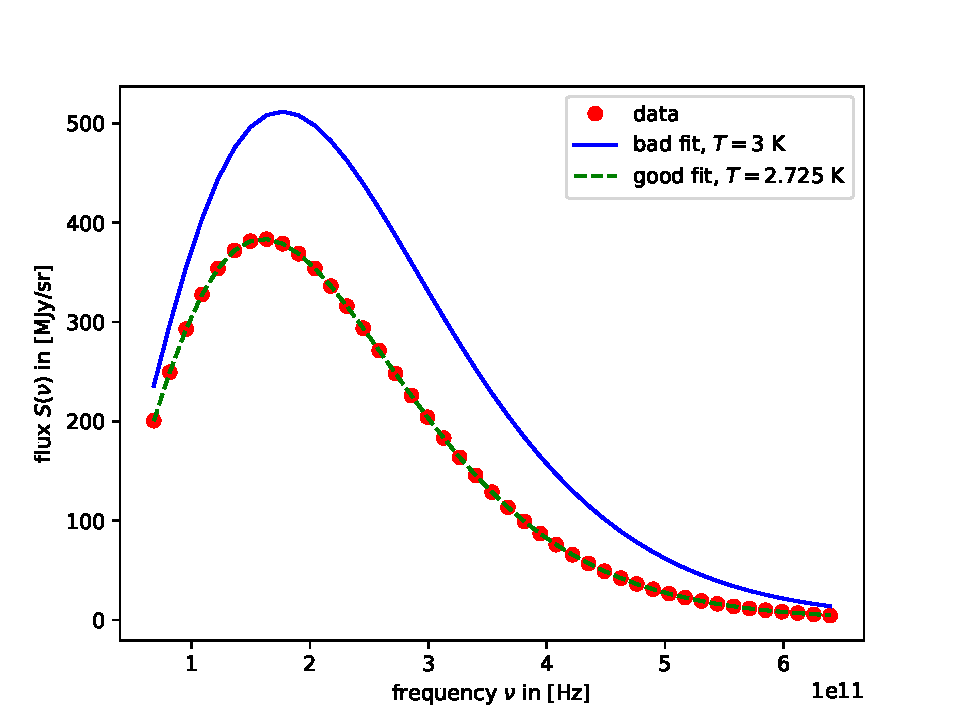
\includegraphics{./figures/planck_plot.pdf}}
\caption{Planck-spectra for different temperatures $T$ superimposed on the COBE-data}
\end{center}
\end{figure}

\item \question{different radiation laws}\\
The script \path{planck_fit.py} does a proper regression of a model $S(\nu,T)$ to the data, by minimising the squared difference between data and model, in units of the noise. There are two models for $S(\nu,T)$, the Planck-spectrum and the simplified Wien-spectrum.
\begin{enumerate}[(a)]
\item{Carry out a fit to the data with both models: What are the temperatures $T$?}
\item{Which model is better at explaining the data?}
\end{enumerate}

\begin{figure}[h]
\begin{center}
\resizebox{9cm}{!}{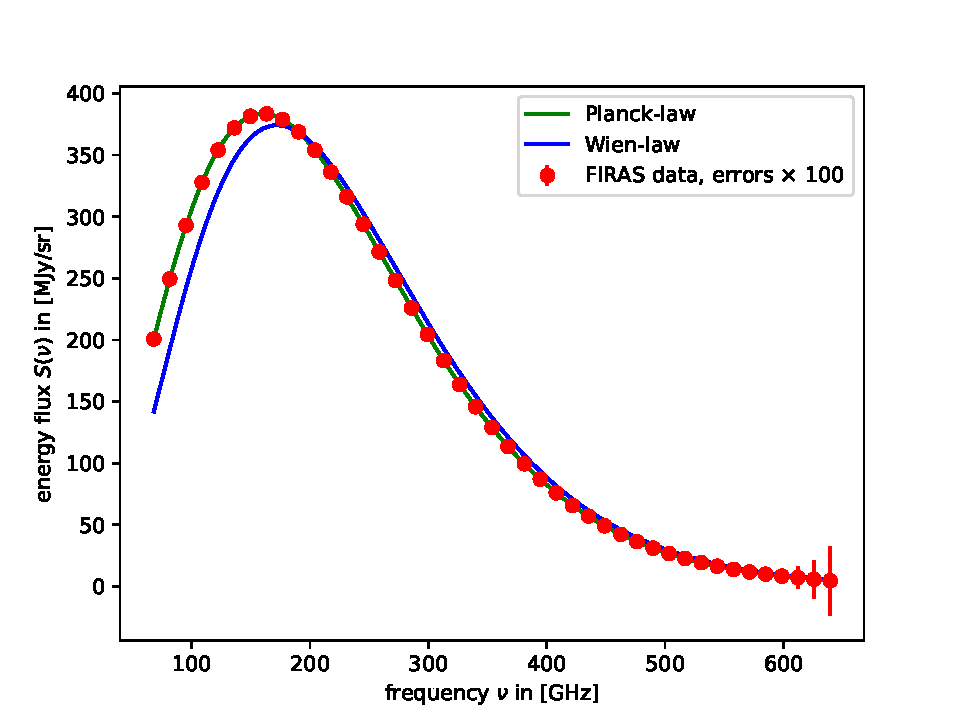
\includegraphics{./figures/planck_fit.pdf}}
\caption{fits of the Planck- and Wien-radiation laws $S(\nu,T)$ to COBE-data}
\end{center}
\end{figure}

\item \question{precision of the measurement}\\
In running the script \path{planck_likelihood.py} you can estimate which range of values for $T$ would be a good fit. It plots the likelihood $\mathcal{L}(T)\propto \exp(-\chi^2(T)/2)$, with 
\begin{equation}
\chi^2(T) = \sum_{i=1}^{n_\mathrm{data}}\left(\frac{S_i-S(\nu_i,T)}{\sigma_i}\right)^2
\end{equation}
for the $n_\mathrm{data}$ data points $S_i$ at the frequencies $\nu_i$. The statistical error is given by the width of the resulting Gauss-curve. Would it be possible to measure the Planck-constant $\hbar$ parallel to the temperature?

\begin{figure}[h]
\begin{center}
\resizebox{9cm}{!}{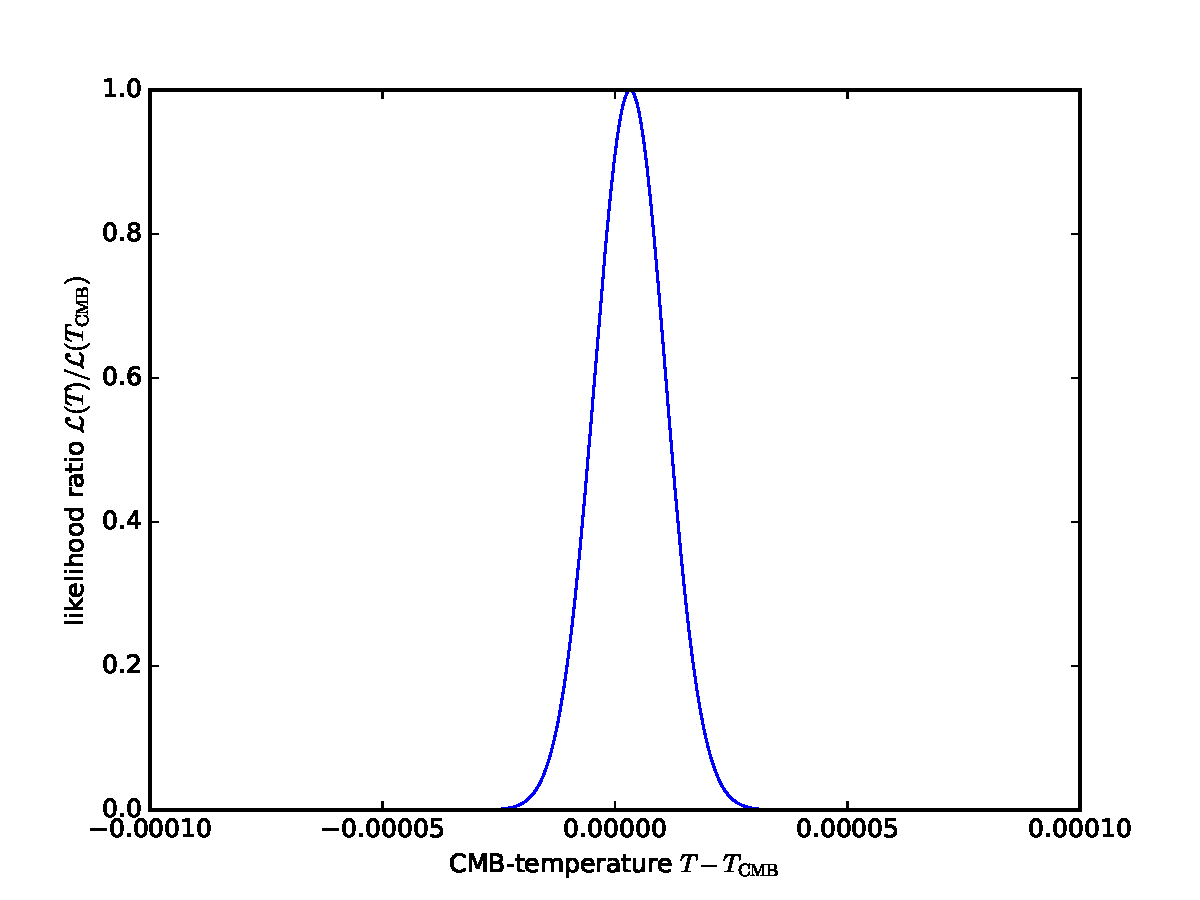
\includegraphics{./figures/planck_likelihood.pdf}}
\caption{likelihood of the CMB-temperature $T$ for the COBE-data}
\end{center}
\end{figure}

\item \question{Solar spectrum}\\
The script \path{solar_plot.py} plots the spectrum of the Sun: Determine the surface temperature $T_\odot$ of the Sun by using Wien's displacement law and the factor that you have determined in the exercises, and estimate the error in your measurement of $T_\odot$.

\end{enumerate}
\end{document}
